\documentclass[aspectratio=169, 12pt]{beamer}

% ── "The Manuscript" Theme — Elite Scholarly Presentation ─────────────────
\usepackage[utf8]{inputenc}
\usepackage[T1]{fontenc}
\usepackage{ebgaramond}   % Core serif for all text
\usepackage{microtype}    % Better kerning/letterspacing
\usepackage{graphicx}
\usepackage{tikz}
\usetikzlibrary{shapes.misc, arrows.meta, positioning, calc}
\usepackage{fontawesome5}
\hypersetup{hidelinks}

% ── Color Palette (Carbon & Cream) ────────────────────────────────────────
\definecolor{Carbon}{HTML}{0a0a0a}       % Near-black background
\definecolor{Cream}{HTML}{fcfcfc}        % Pure off-white text
\definecolor{MutedGold}{HTML}{a16207}    % Dark professional gold
\definecolor{SlateGrey}{HTML}{444444}    % Subtle boundaries

\setbeamercolor{background canvas}{bg=Carbon}
\setbeamercolor{normal text}{fg=Cream}
\setbeamercolor{frametitle}{fg=Cream}
\setbeamercolor{title}{fg=Cream}
\setbeamercolor{item}{fg=Cream}

% ── Minimalist Layout ──────────────────────────────────────────────────────
\setbeamertemplate{navigation symbols}{}
\setbeamertemplate{headline}{}
\setbeamertemplate{footline}{
  \hfill\small\textcolor{MutedGold}{\insertframenumber\,/\,\inserttotalframenumber}\quad\vspace{6pt}
}

% ── Typography ─────────────────────────────────────────────────────────────
\setbeamerfont{frametitle}{family=\ebgaramond, series=\bfseries, size=\Large}
\setbeamerfont{title}{family=\ebgaramond, series=\bfseries, size=\Huge}

% ── Helpers ──────────────────────────────────────────────────────────────────
\newcommand{\citepoint}[1]{\textcolor{MutedGold}{\textsf{#1}}}
\newcommand{\emphasis}[1]{\textcolor{Cream}{\textbf{#1}}}
\newcommand{\subtle}[1]{\textcolor{SlateGrey}{#1}}
\newcommand{\analogy}[2]{
    \begin{center}
    \begin{tikzpicture}
        \node[draw=MutedGold, thick, rounded corners=2pt, inner sep=10pt, fill=Carbon, text width=0.85\textwidth, align=center] {
            \citepoint{\faLightbulb}\quad \textit{``#1 is like #2''}
        };
    \end{tikzpicture}
    \end{center}
}

% ════════════════════════════════════════════════════════════════════════════
\begin{document}

% 1. TITLE
\begin{frame}[plain]
    \centering
    \vfill
    {\Huge\ebgaramond\bfseries Why Algorithms Need the Machine}\\[0.5em]
    {\large\textit{Locality, Speed, and the 16-Structure Sprint}}\\[2.5em]
    
    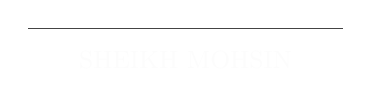
\begin{tikzpicture}
        \draw[SlateGrey, line width=0.3pt] (-2,0) -- (2,0);
        \node[Cream, font=\small\ebgaramond] at (0,-0.4) {SHEIKH MOHSIN};
    \end{tikzpicture}
    
    \vfill
    {\footnotesize\textcolor{SlateGrey}{Systems Programming | April 2026 | Prof. Sanjay Patel}}
\end{frame}

% 2. THE SPATIAL PREMISE (RESTORED)
\begin{frame}{The Spatial Premise}
    \vspace{1.5em}
    \begin{columns}[c]
        \column{0.55\textwidth}
        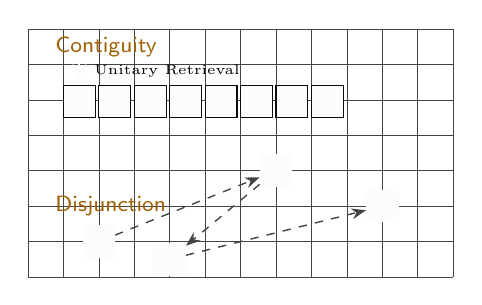
\begin{tikzpicture}[x=0.45cm, y=0.45cm]
            \draw[SlateGrey, line width=0.2pt, step=1] (-1, -3) grid (11, 4);
            

            % Contiguous Case
            \node[anchor=west, font=\footnotesize] at (-0.5, 3.5) {\citepoint{Contiguity}};
            \foreach \i in {0,...,7} {
                \draw[fill=Cream, draw=Carbon] (\i, 1.5) rectangle (\i+0.9, 2.4);
            }
            \draw[Cream, -{Stealth}, line width=0.8pt] (0.45, 3.1) -- (0.45, 2.5);
            \node[font=\tiny, anchor=west] at (0.6, 2.8) {Unitary Retrieval};


            % Disjoint Case
            \node[anchor=west, font=\footnotesize] at (-0.5, -1) {\citepoint{Disjunction}};
            \node[draw=Cream, fill=Cream, minimum size=0.4cm] (p1) at (1, -2) {};
            \node[draw=Cream, fill=Cream, minimum size=0.4cm] (p2) at (6, 0) {};
            \node[draw=Cream, fill=Cream, minimum size=0.4cm] (p3) at (3, -2.5) {};
            \node[draw=Cream, fill=Cream, minimum size=0.4cm] (p4) at (9, -1) {};
            \draw[SlateGrey, -{Stealth}, line width=0.5pt, dashed] (p1) -- (p2);
            \draw[SlateGrey, -{Stealth}, line width=0.5pt, dashed] (p2) -- (p3);
            \draw[SlateGrey, -{Stealth}, line width=0.5pt, dashed] (p3) -- (p4);
        \end{tikzpicture}

        \column{0.4\textwidth}
        \begin{itemize}
            \item Modern CPUs operate on a \emphasis{spatial premise}.
            \item Contiguous layouts leverage hardware prefetching.
            \item Pointer-chasing induces serial stalls.
            \item Memory latency is the \emphasis{primary bottleneck} of the 21st-century.
        \end{itemize}
    \end{columns}
\end{frame}

% 3. OVERVIEW OF Project 
\begin{frame}{The Scale of the Project}
    \vfill
    \begin{columns}[T]
        \column{0.3\textwidth}
        \centering
        \citepoint{\Huge 16}\\
        \subtle{Data Structural\\Families}
        
        \column{0.3\textwidth}
        \centering
        \citepoint{\Huge 6,641}\\
        \subtle{High-Fidelity\\Datapoints}
        
        \column{0.3\textwidth}
        \centering
        \citepoint{\Huge 722.2B}\\
        \subtle{Memory Elements\\Analyzed}
    \end{columns}
    \vfill
    
\end{frame}

% 2. THE ANALOGY (CORE PREMISE)
\begin{frame}{The Reality: Big O is Only Half the Story}
    \vspace{1em}
    Most students learn algorithms as a count of "steps." Hardware is different.
    \vspace{0.5em}
    \analogy{Memory Access}{a Coffee Shop vs. a Warehouse}
    \begin{columns}[T]
        \column{0.48\textwidth}
        \citepoint{L1 Cache (Coffee Shop)}\\
        Right in front of you. Fast. Automatic.
        
        \column{0.48\textwidth}
        \citepoint{RAM (The Warehouse)}\\
        Slow. Requires a trip. CPU stalls while waiting.
    \end{columns}
    \vfill
    \centering
    \textit{Choosing a data structure that "keeps data close" is the secret to speed.}
\end{frame}

% 3. NEW DATA STRUCTURES
\begin{frame}{Meet the Contenders: Beyond the BST}
    How do we organize data when a simple list isn't enough?
    \vspace{1em}
    \begin{columns}[T]
        \column{0.32\textwidth}
        \citepoint{SkipList}\\
        \emphasis{The Express Elevator}\\
        {\footnotesize A list with "shortcut" lanes to skip nodes. Fast as a Tree, but simpler.}

        \column{0.32\textwidth}
        \citepoint{vEB Tree}\\
        \emphasis{Digital Fractals}\\
        {\footnotesize Uses recursion to divide data into clusters. Theoretically the fastest.}

        \column{0.32\textwidth}
        \citepoint{B-Tree}\\
        \emphasis{The Librarian}\\
        {\footnotesize Stores hundreds of items per node. Keeps the CPU happy by minimizing trips.}
    \end{columns}
    \vfill
    {\footnotesize\textit{Measured all 16 contenders across 5 orders of magnitude.}}
\end{frame}

% 4. THE SPEED RANKING
\begin{frame}{Who Wins the Sprint? (N = 41 Million)}
    \begin{columns}[c]
        \column{0.68\textwidth}
        \centering
        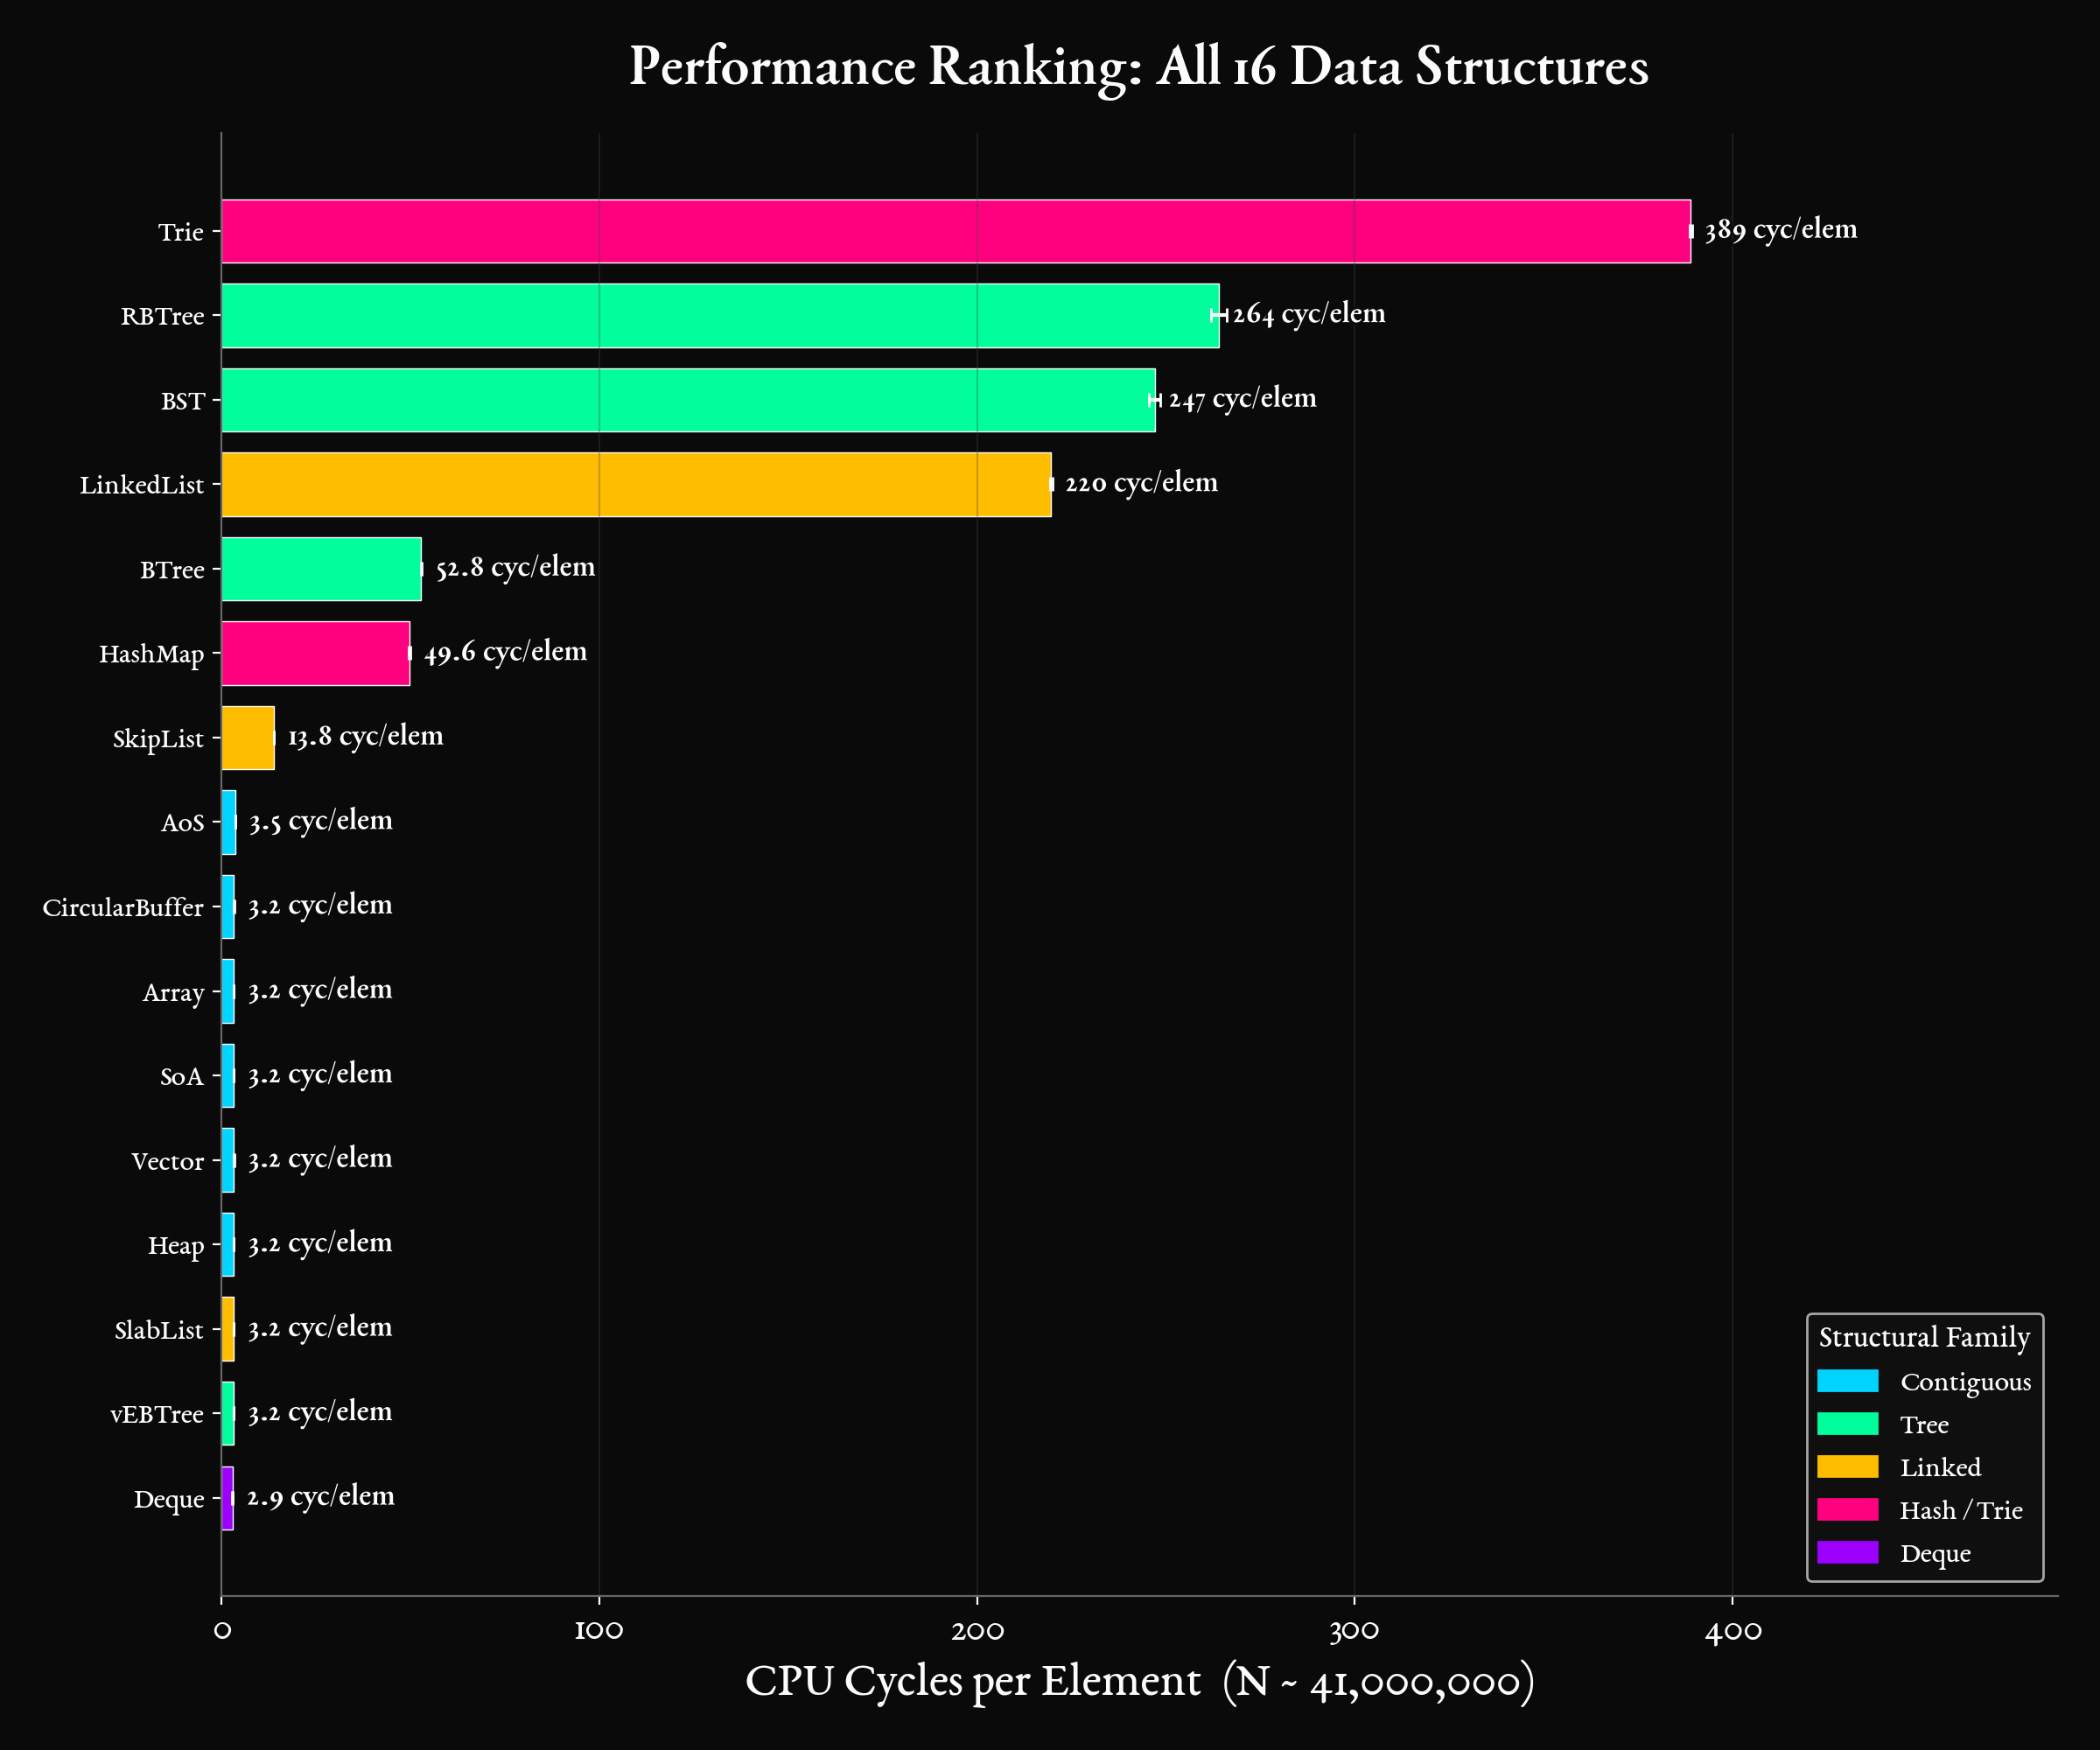
\includegraphics[height=0.75\textheight]{slides/fig_fastest.png}
        
        \column{0.3\textwidth}
        \citepoint{The Latency Gap}\\
        \vfill
        {\small 
        \emphasis{Arrays} win by 40x.
        \vfill
        \subtle{Linked structures stay in "the warehouse" while the CPU waits.}
        }
    \end{columns}
\end{frame}

% 5. THE CACHE CLIFF
\begin{frame}{Size Matters: The Cache Cliff}
    \centering
    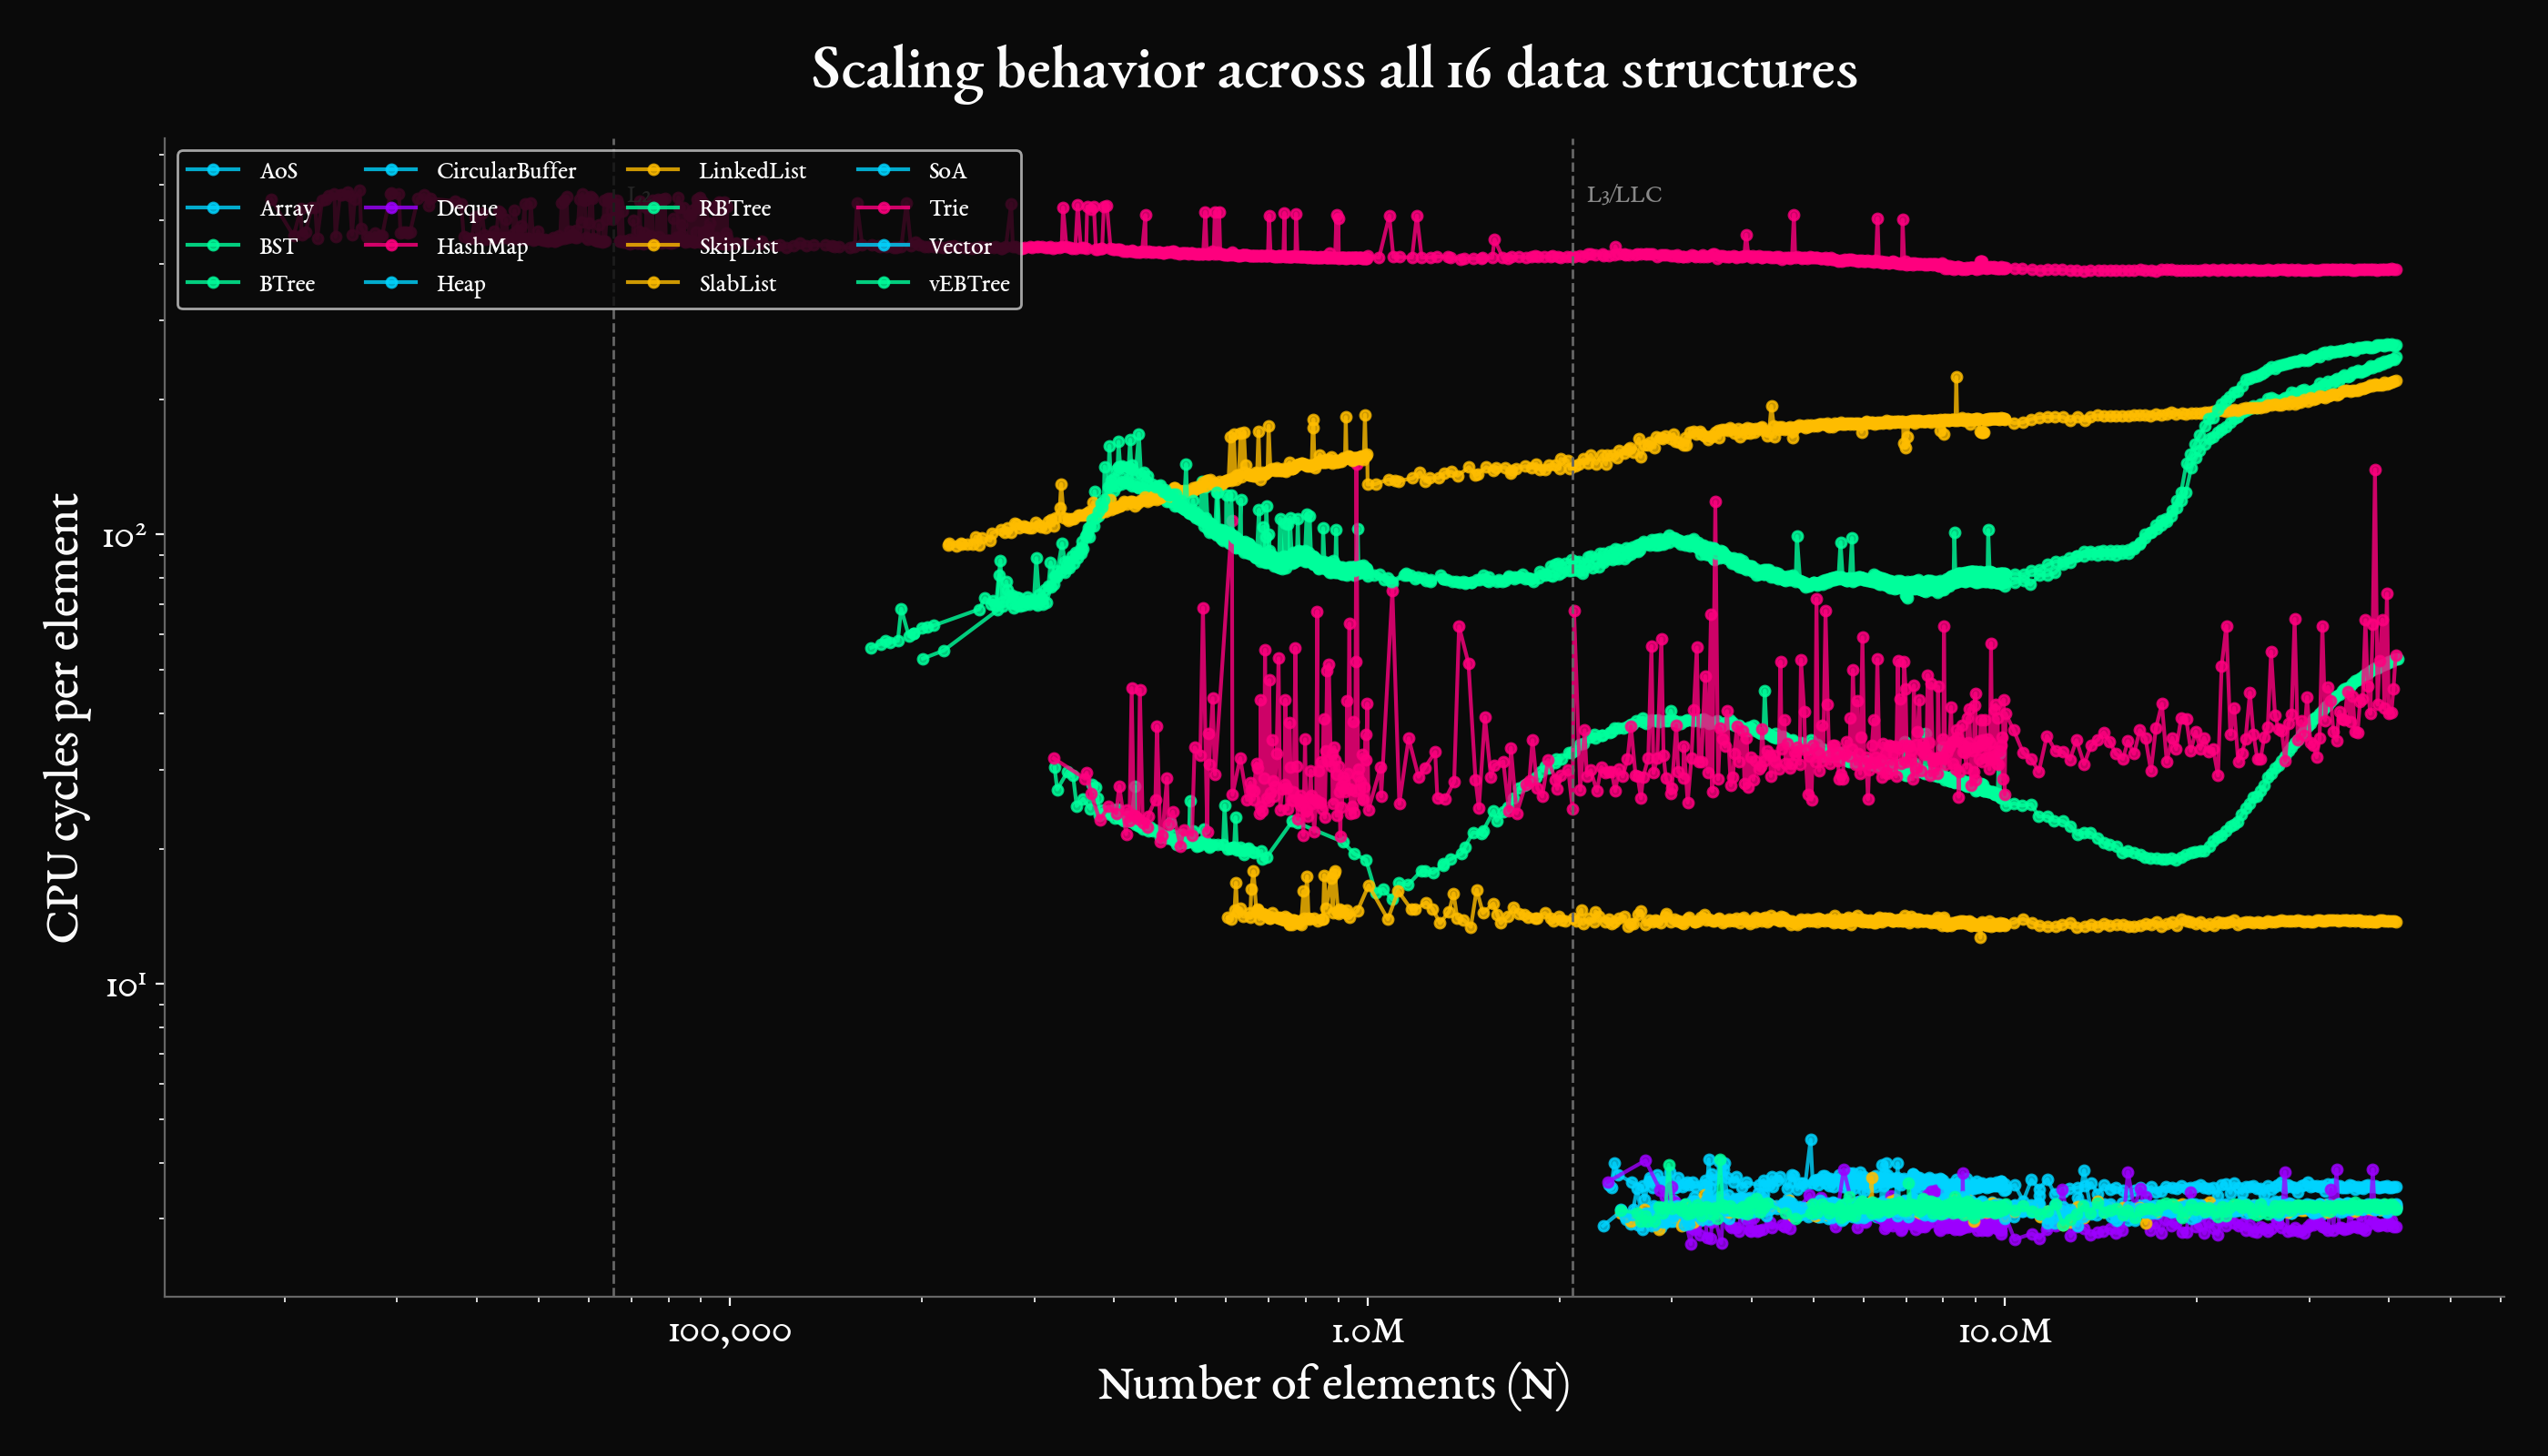
\includegraphics[width=0.85\textwidth]{slides/fig_scaling.png}\\[0.5em]
    {\footnotesize Notice the "step up" in cycles as data outgrows the CPU's internal memory.}
\end{frame}

% 6. WHY ARRAYS WIN
\begin{frame}{The Secret Multiplier: Locality}
    \begin{columns}[c]
        \column{0.45\textwidth}
        \centering
        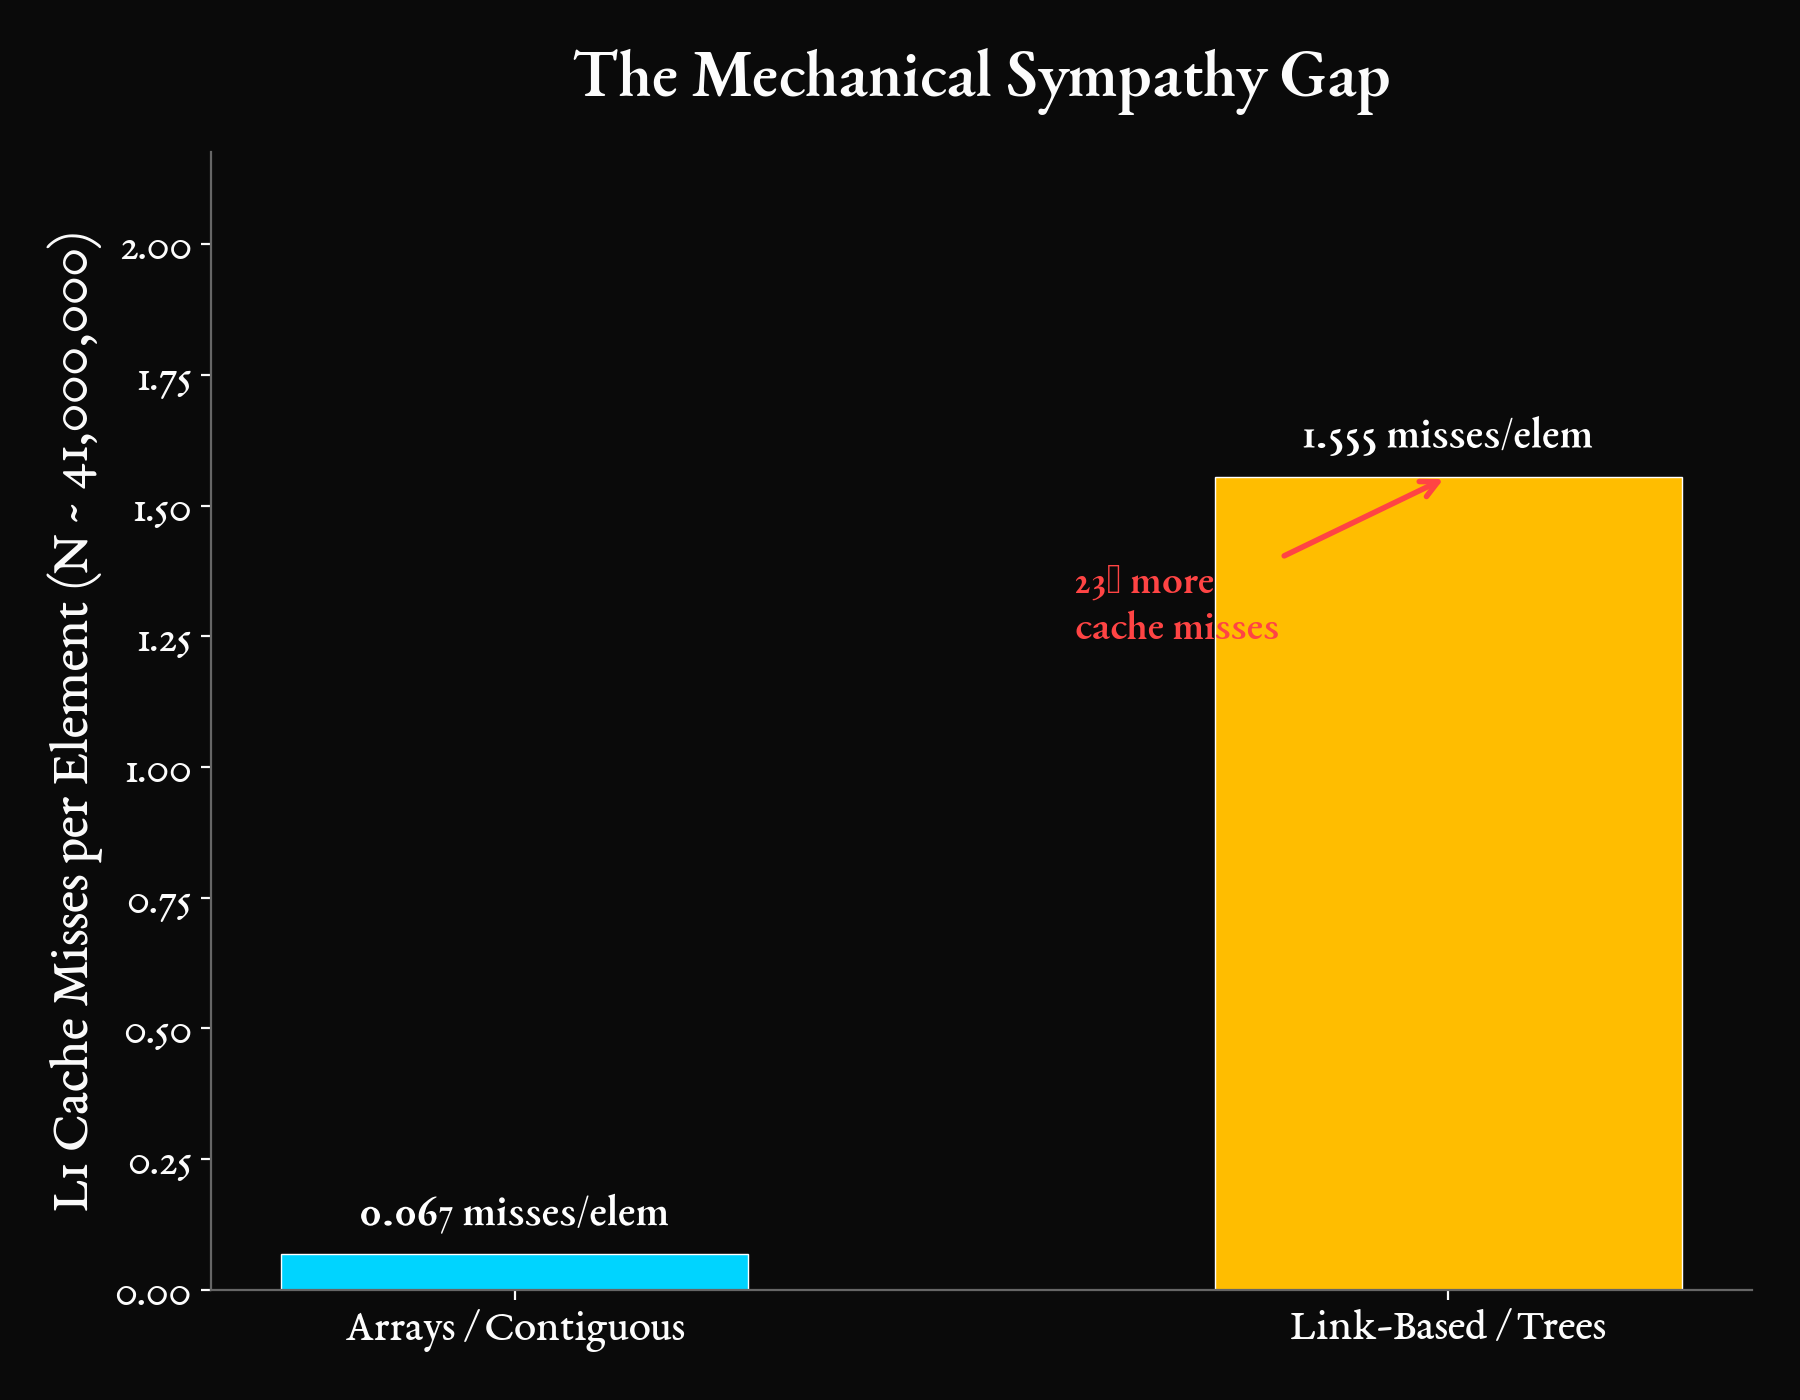
\includegraphics[width=\textwidth]{slides/fig_why_arrays.png}
        
        \column{0.5\textwidth}
        \analogy{Locality}{Shopping in one aisle vs. running across the store.}
        \vspace{1em}
        {\small 
        \emphasis{Pointer Tax:} Lists force the CPU to find a new address for every single element.}
    \end{columns}
\end{frame}

% 7. PRACTICAL WISDOM
\begin{frame}{Practical Lessons}
    \centering
    \vfill
    {\Large\citepoint{Algorithms are Math, but Performance is Physics.}}\\[2.5em]
    
    \begin{itemize}
        \item[] \citepoint{I.} \emphasis{Contiguity is King:} Keep your data together in memory.
        \item[] \citepoint{II.} \emphasis{Complexity $\neq$ Speed:} A smart algorithm can be slow if it's "messy."
        \item[] \citepoint{III.} \emphasis{Hardware Harmony:} Think about the machine, not just the code.
    \end{itemize}
    \vfill
\end{frame}
% 8. Q&A
\begin{frame}[plain]
    \centering
    \vfill
    {\Huge\citepoint{\faChartLine}}\\[1em]
    {\Huge\ebgaramond\bfseries Any Questions?}\\[2.5em]
    
    
    \vfill
\end{frame}

% 9. THANK YOU
\begin{frame}[plain]
    \centering
    \vfill
    {\Huge\ebgaramond\bfseries Thank You!}\\[1.5em]
    {\large\citepoint{Sheikh Mohsin}}\\[0.5em]
    {\small\subtle{Systems Programming | 2026}}\\[2.5em]
    
    \begin{tikzpicture}
        \draw[SlateGrey, line width=0.3pt] (-3,0) -- (3,0);
    \end{tikzpicture}\\[1em]
    \faGithub\ \ \href{https://github.com/SheikhMohsin9311/Performance-and-Data-Representation}{\texttt{github.com/SheikhMohsin9311/Performance-and-Data-Representation}}
\end{frame}
\end{document}